\begin{Oplossing}{1.1}
De defintie op Wikipedia klopt volgens ons niet helemaal. Het eerste Fibonaccigetal is niet 0, maar 1. Het tweede Fibonaccigetal is ook 1. Daarna is het n-de Fibonaccigetal gelijk aan de som van de twee vorige. De code in listing~\ref{recfibo} is kort, maar nogal onefficiënt. Om het 100ste getal te berekenen, moeten we eerst het 99ste en het 98ste getal berekenen en die optellen. Om het 99ste te berekenen moeten we echter opnieuw eerst het 98ste berekenen. We doen dus veel te veel werk.
\begin{lstlisting}[caption={Recursieve methode om Fibonacci-getallen te berekenen}, label=recfibo]
public static int fibonacci(int getal) {
	if (getal <= 0)
		throw new IllegalArgumentException();
	if (getal <= 2)
		return 1;
	else
		return fibonacci(getal - 1) + fibonacci(getal - 2);
}
\end{lstlisting}
\end{Oplossing}
\begin{Oplossing}{1.2}
\begin{lstlisting}[caption={Recursieve methode om de som van de cijfers van een getal te berekenen}, label=recsomgetallen]
public static int somVanCijfers(int getal) {
	getal = Math.abs(getal);
	if (getal < 10) //basisgeval, slechts 1 cijfer
		return getal;
	else //getal bestaat uit meer dan 1 cijfer, recursieve oproep van de functie nodig
		return getal % 10 + somVanCijfers(getal / 10);
}
\end{lstlisting}
\end{Oplossing}
\begin{Oplossing}{1.3}
Een vraag die we geregeld krijgen in de oefenzitting is waarom het niet werkt als de test of de gegeven string null is, later in de code staat, bvb. na de test of de lengte van de string kleiner of gelijk is aan 1. Wat gebeurt er als je de lengte vraagt van een niet bestaande string? In plaats van \verb+charAt+ kan je vanzelfsprekend ook gebruik maken van \verb+substring+.
\begin{lstlisting}[caption={Recursieve methode om een string om te keren}, label=reckeerom]
public static String keerOm(String s) {
	if (s == null)
		throw new IllegalArgumentException();
	else if (s.length() <= 1)
		return s;
	else
		return s.charAt(s.length() - 1) + Recursie.keerOm(s.substring(0, s.length() - 1));
}
\end{lstlisting}
\end{Oplossing}
\begin{Oplossing}{1.4}
Deze methode is eigenlijk veel eenvoudiger als een lus te programmeren, maar het kan ook recursief. Merk de ternaire operator \verb+( ? : )+ in de laatste return op. Je kan die altijd vervangen door een toekenning in een \verb+if else+, maar deze ternaire operator is een stuk korter.
\begin{lstlisting}[caption={Recursieve methode om het aantal keer te tellen dat de letter x in een string voorkomt}, label=reccountx]
public static int countX(String s) {
	if (s == null)
		throw new IllegalArgumentException();
	else if (s.length() == 0)
		return 0;
	else
		return ((s.charAt(0) == 'x') ? 1 : 0) + countX(s.substring(1));
}
\end{lstlisting}

\end{Oplossing}
\begin{Oplossing}{1.5}
Een aandachtspunt (wat je ongetwijfeld weet vanuit het eerste semester, maar misschien wel even vergeten was) is het vergelijken van strings. Kom niet in de verleiding om \verb+==+ te gebruiken, maar doe dit altijd met de methode \verb+equals+. Weet je nog waarom?
\begin{lstlisting}[caption={Recursieve methode om het aantal keer te tellen dat de string hi in een string voorkomt}, label=reccounthi]
public static int countHi(String s) {
	if (s == null)
		throw new IllegalArgumentException();
	else if (s.length() <= 1)
		return 0;
	else {
		if ((s.substring(0, 2)).equals("hi")) {
			return 1 + countHi(s.substring(2));
		} else
			return countHi(s.substring(1));
	}
}
\end{lstlisting}
\end{Oplossing}
\begin{Oplossing}{1.6}
\begin{lstlisting}[caption={Vervang in een string elke letter x door een y}, label=recchangexy]
public static String changeXY(String s) {
	if (s == null)
		throw new IllegalArgumentException();
	if (s.length() == 0)
		return s;
	else
		return ((s.charAt(0) == 'x' ? "y" : s.charAt(0)) + changeXY(s.substring(1)));
}
\end{lstlisting}
\end{Oplossing}
\begin{Oplossing}{1.7}
\begin{lstlisting}[caption={Vervang in een string elke pi door een 3.14}, label=recchangepi]
public static String changePi(String s) {
	if (s == null)
		throw new IllegalArgumentException();
	if (s.length() <= 1)
		return s;
	else {
		if ((s.substring(0, 2)).equals("pi")) {
			return "3.14" + Recursie.changePi(s.substring(2));
		} else
			return s.charAt(0) + Recursie.changePi(s.substring(1));
	}
}
\end{lstlisting}
\end{Oplossing}
\begin{Oplossing}{1.8}
\begin{lstlisting}[caption={Tweelog van een macht van twee}, label=rectweelog]
public static int tweelog(int getal) {
	if (getal <= 0)
		throw new IllegalArgumentException();
	if (getal == 1)
		return 0;
	else
		return 1 + tweelog(getal / 2);
}
\end{lstlisting}
\end{Oplossing}
\begin{Oplossing}{1.9}
Ook voor deze oefening ligt het meer voor de hand om een lus te gebruiken, maar het kan dus ook recursief.
\begin{lstlisting}[caption={Maximum van een lijst getallen}, label=recfindmaximum]
public static double findMaximum(List<Double> lijst) {
	if (lijst == null || lijst.size() == 0)
		throw new IllegalArgumentException();
	else if (lijst.size() == 1)
		return lijst.get(0);
	else {
		double g = findMaximum(lijst.subList(1, lijst.size()));
		if (lijst.get(0) > g)
			return lijst.get(0);
		else
			return g;
	}
}
\end{lstlisting}
\end{Oplossing}
\begin{Oplossing}{1.10}
Ongetwijfeld de moeilijkste oefening, ook al omdat je nu moet werken met lijsten.
\begin{lstlisting}[caption={Alle substrings van een gegeven string}, label=recfindsubstrings]
public static ArrayList<String> findSubstrings(String string) {
	if (string == null)
		throw new IllegalArgumentException();
	ArrayList<String> res = new ArrayList<String>();
	if (string.length() <= 1) { //ook de lege string telt mee!
		res.add(string);
		return res;
	}
	else {
		res.add(string.substring(0, 1));
		ArrayList<String> res2 = findSubstrings(string.substring(1));
		res.addAll(res2);
		for (String s : res2) {
			res.add(string.charAt(0) + s);
		}
		return res;
	}
}
\end{lstlisting}
\end{Oplossing}
\begin{Oplossing}{1.11}
\begin{lstlisting}[caption={Aantal kaarten nodig om een kaartenhuisje te maken}, label=reckaartenHuisje]

public class Kaartenhuisje {

	public static void main(String[] args) {
		for (int n = 1 ; n <= 20 ; n++)
		System.out.println("Aantal Kaarten nodig voor een kaarten huisje van " + n +
			" verdieping" + (n == 1 ? " = ": "en = ") + aantalKaarten(n));
	}
	
	private static int aantalKaarten(int n){
		if (n < 1) throw new IllegalArgumentException();
		if (n == 1) return 2;
		else return aantalKaarten(n-1) + (n-1) + 2 * n ;
	}

}
\end{lstlisting}

\end{Oplossing}
\begin{Oplossing}{2.1}

\begin{oefenumerate}
	\item Ja want elke knoop in deze boom heeft maximaal 2 kinderen.
	\item Knoop F.
	\item Het maximaal aantal knopen van een pad van de wortel naar
een blad is vier, dus de diepte van deze boom is vier.
	\item Neen, niet compleet.
Alle niveaus behalve eventueel de laatste zijn niet
volledig gevuld. Zo ontbreekt er een knoop op niveau 3:
het linkerkind van knoop G.
Verder zijn alle knopen op het laatste niveau ook niet
aan de linkerzijde: de twee kinderen van knoop A ontbreken.
	\item Knopen A, C, E en H.
	\item Knopen F, B, D, G en I.
	\item Deze subboom bevat 5 knopen.
	\item F B A D C E G I H
	\item A B C D E F G H I
	\item A C E D B H I G F

	
\end{oefenumerate}
\end{Oplossing}
\begin{Oplossing}{2.2}
\begin{oefenumerate}
\item
\item
\item Figuur~\ref{fig:binboomopgave} toont een grafische voorstelling van de gegeven boom.
\begin{figure}[htbp]
    \centering
\begin{tikzpicture}[every node/.style={},
				level 1/.style={sibling distance=40mm},
				level 2/.style={sibling distance=20mm},
				level 3/.style={sibling distance=10mm}]]
\node {C}
child { node {A}
	child { node {D} }
	child { node {F} }
}
child { node {G}
	child {node {E}
		child { node {H}}
		child[missing]}
	child { node {B}}};		
\end{tikzpicture}
\caption{Boom uit oefening 2}
    \label{fig:binboomopgave}
\end{figure}
\item Een preorder doorloop geeft: C A D F G E H B.
\item
\item De code van de boom uit oefening 1 kan er als volgt uitzien:
\begin{lstlisting}[caption={Binaire boom uit oefening 1}, label=binoef1]
package ui;

import domain.BinaryTree;

public class BinaryTreeDriver2 {

	public static void main(String[] args) {
		//begin bij de bladeren ...
		BinaryTree<String> nodeA = new BinaryTree<>("A");
		BinaryTree<String> nodeC = new BinaryTree<>("C");
		BinaryTree<String> nodeE = new BinaryTree<>("E");
		BinaryTree<String> nodeH = new BinaryTree<>("H");

		// ... ga vervolgens naar alle interne knopen ...
		// knoop I heeft links H en rechts niets
		BinaryTree<String> nodeI = new BinaryTree<>("I",nodeH, null);
		// knoop G heeft links niets en rechts I
		BinaryTree<String> nodeG = new BinaryTree<>("G",null, nodeI);
		// knoop D heeft links C en rechts E
		BinaryTree<String> nodeD = new BinaryTree<>("D",nodeC,nodeE);
		// knoop B heeft links A en rechts D
		BinaryTree<String> nodeB = new BinaryTree<>("B",nodeA, nodeD);
		
		// ... en eindig met de wortel
		// boom heeft root F en heeft links B en rechts G
		BinaryTree<String> boom = new BinaryTree<>("F",nodeB, nodeG);
		boom.printPreorder();
	}

}
 \end{lstlisting}

 \item F B A D C E G I H
\end{oefenumerate}

\end{Oplossing}
\begin{Oplossing}{2.3}
In het \verb+domain+ package voeg je in \verb+BinaryTree.java+ volgende methode in:
\begin{lstlisting}[caption={In-order doorloop van een binaire boom}, label=bininorder]
public void printInorder(){
	if (this.leftTree != null) {
		this.leftTree.printInorder();
	}
	System.out.print(this.data + " ");
	if (this.rightTree != null) {
		this.rightTree.printInorder();
	}
}
\end{lstlisting}

\end{Oplossing}
\begin{Oplossing}{2.4}
In het \verb+domain+ package voeg je in \verb+BinaryTree.java+ volgende methode in:
\begin{lstlisting}[caption={Post-order doorloop van een binaire boom}, label=binpostorder]
public void printPostorder(){
	if (this.leftTree != null) {
		this.leftTree.printPostorder();
	}
	if (this.rightTree != null) {
		this.rightTree.printPostorder();
	}
	System.out.print(this.data + " ");
}
\end{lstlisting}
\end{Oplossing}
\begin{Oplossing}{2.5}
Je vindt het correcte aantal knopen (9) bvb. met de methode \verb+countNodes+ die je implementeert in \verb+BinaryTree.java+. Vanzelfsprekend kan je met \verb+if+ constructies werken, maar de \emph{ternaire operator} van java maakt de code wel een stuk kernachtiger (listing~\ref{bincountnodes}).
\begin{lstlisting}[caption={Tel het aantal knopen in een binaire boom}, label=bincountnodes]
public int countNodes() {
	return 1 + (this.leftTree == null ? 0 : this.leftTree.countNodes())
					+ (this.rightTree == null ? 0 : this.rightTree.countNodes());
}
\end{lstlisting}
\end{Oplossing}
\begin{Oplossing}{2.6}
Je vindt de maximale diepte van een boom met de methode \verb+getMaxDepth+ die je implementeert in \verb+BinaryTree.java+. Ook hier weer een oplossing met de \emph{ternaire operator} van java (listing~\ref{bingetmaxdepth}).
\begin{lstlisting}[caption={De diepte van een binaire boom}, label=bingetmaxdepth]
public int getDepth() {
	return 1 + Math.max((this.leftTree == null ? 0 : this.leftTree.getDepth()),
					(this.rightTree == null ? 0 : this.rightTree.getDepth()));
}
\end{lstlisting}

\end{Oplossing}
\begin{Oplossing}{2.7}
Listing~\ref{binisleaf} toont een eenvoudige implementatie voor deze functie.
\begin{lstlisting}[caption={Is een knoop een blad?}, label=binisleaf]
public boolean isLeaf() {
	return this.leftTree == null && this.rightTree == null;
}
\end{lstlisting}
\end{Oplossing}
\begin{Oplossing}{2.8}
Listing~\ref{bincountleaves} toont een eenvoudige implementatie voor deze functie.
\begin{lstlisting}[caption={Hoeveel bladeren bevat deze boom?}, label=bincountleaves]
public int countLeaves() {
	if (this.isLeaf()) {
		return 1;
	} else {
		return (this.leftTree == null ? 0 : this.leftTree.countLeaves())
					+ (this.rightTree == null ? 0 : this.rightTree.countLeaves());
	}
}
\end{lstlisting}
\end{Oplossing}
\begin{Oplossing}{2.9}
Deze methode is wat moeilijker dan de vorige omdat je nu met lijsten moet werken. Listing~\ref{bingetdataleaves} toont een mogelijke implementatie. Met een lus in de \verb+main+ methode kan je als test de data van alle bladeren uitschrijven.
\begin{lstlisting}[caption={Genereer een lijst met de data van alle bladeren}, label=bingetdataleaves]
public ArrayList<E> getDataLeaves() {
	ArrayList<E> res = new ArrayList<>();
	if (this.isLeaf()) {
		res.add(this.data);
	} else {
		res = (this.leftTree == null ? new ArrayList<>() : this.leftTree.getDataLeaves());
		ArrayList<E> rightLeaves =
			(this.rightTree == null ? new ArrayList<>() : this.rightTree.getDataLeaves());
		res.addAll(rightLeaves);
	}
	return res;
}
\end{lstlisting}

\end{Oplossing}
\begin{Oplossing}{2.10}
Een mogelijke implementatie vind je in listing~\ref{bincontains}.
\begin{lstlisting}[caption={Komt een bepaalde waarde voor in een boom?}, label=bincontains]
public boolean contains(E s) {
	if (s == null) {
		return false;
	}
	if (s.equals(this.data)) {
		return true;
	} else {
		return (this.leftTree == null ? false : this.leftTree.contains(s)) ||
				(this.rightTree == null ? false : this.rightTree.contains(s));
	}
}
\end{lstlisting}

\end{Oplossing}
\begin{Oplossing}{3.1}
De eerste boom (figuur~\ref{fig:BSToef1}) is een BST omdat elke knoop (alfabetisch) groter is dan alle knopen in de linkersubboom en kleiner dan alle knopen in de rechtersubboom. De tweede boom (figuur~\ref{fig:oefBST2}) is echter geen BST omdat 3 niet groter is dan 4 (terwijl de knoop 4 toch in de linkersubboom zit).
\end{Oplossing}
\begin{Oplossing}{3.2}
We bekijken nog eens de definitie van binaire zoekboom: voor elke knoop in de boom geldt dat zijn waarde strikt groter is dan alle waarden in zijn linkersubboom en strikt kleiner dan alle waarden in zijn rechtersubboom. Deze volgorde is ook wat een in-order doorloop doet.
\end{Oplossing}
\begin{Oplossing}{3.3}
Er is maar één mogelijke oplossing, nl. figuur~\ref{fig:oefBST39opl}.
\begin{figure}[htbp]
    \centering
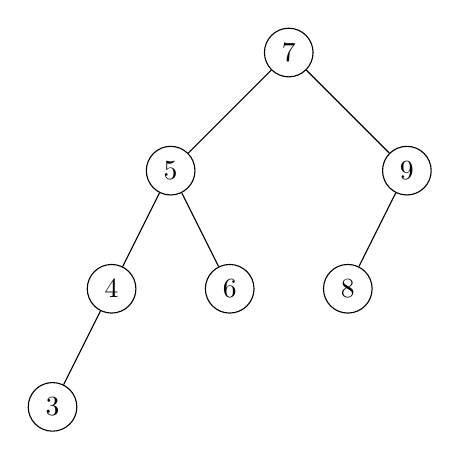
\begin{tikzpicture}[every node/.style={circle,draw},
			level 1/.style={sibling distance=30mm},
			level 2/.style={sibling distance=15mm},]
\node {7}
child { node {5}
	child { node {4 }
		child { node {3}}
		child[missing]}
	child { node {6} }
	}
child { node {9}
	child { node {8}}
	child[missing]
	};
\end{tikzpicture}
\caption{Getallen van 3 t.e.m. 9 invullen in de knopen}
    \label{fig:oefBST39opl}
\end{figure}
\end{Oplossing}
\begin{Oplossing}{3.4}
De \verb+main+ methode construeert de (gebalanceerde) BST uit figuur~\ref{fig:oefBSTmain}.
\begin{figure}[htbp]
    \centering
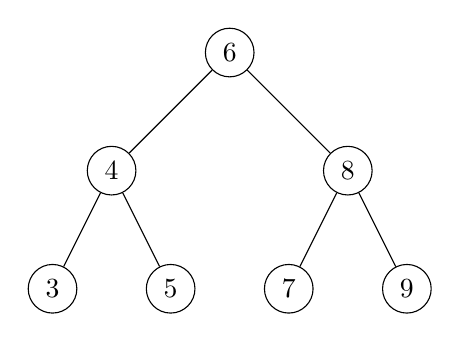
\begin{tikzpicture}[every node/.style={circle,draw},
			level 1/.style={sibling distance=30mm},
			level 2/.style={sibling distance=15mm},]
\node {6}
child { node {4}
	child { node {3}}
	child { node {5}}
	}
child { node {8}
	child { node {7}}
	child { node {9}}
	};
\end{tikzpicture}
\cprotect\caption{ResultaatBST van de \verb+main+ methode}
    \label{fig:oefBSTmain}
\end{figure}
\begin{lstlisting}[caption={addNode(data) methode}, label=bstaddnode]
public boolean addNode(E data) {
	if (data == null) {
		throw new IllegalArgumentException();
	}
	if (this.data.compareTo(data) == 0) {
		return false; //geen twee keer zelfde data in BST
	} else if (this.data.compareTo(data) > 0) {//ga naar linkersubboom
		if (this.leftTree == null) {
			this.leftTree = new BinarySearchTree<>(data);
			return true;
		} else return (this.leftTree.addNode(data));
	} else if (this.rightTree == null) {
		this.rightTree = new BinarySearchTree<>(data);
		return true;
	} else return (this.rightTree.addNode(data));
}
\end{lstlisting}

\end{Oplossing}
\begin{Oplossing}{3.5}
\begin{lstlisting}[caption={lookUp(data) methode}, label=bstlookUp]
public boolean lookup(E data) {
	if (data == null) {
		return false;
	}
	if (this.data.compareTo(data) == 0) {
		return true;
	} else {
		if (this.data.compareTo(data) > 0) {
			return (this.leftTree == null ? false : this.leftTree.lookup(data));
		} else {
			return (this.rightTree == null ? false : this.rightTree.lookup(data));
		}
	}
}
\end{lstlisting}
\end{Oplossing}
\begin{Oplossing}{3.6}
\begin{lstlisting}[caption={searchGreatest methode}, label=bstsearchgreatest]
public E searchGreatest() {
	if (this.rightTree == null) {
		return this.data;
	} else {
		return this.rightTree.searchGreatest();
	}
}
 \end{lstlisting}

\end{Oplossing}
\begin{Oplossing}{3.7}
\begin{lstlisting}[caption={searchSmallest methode}, label=bstsearchsmallest]
public E searchSmallest() {
	if (this.leftTree == null) {
		return this.data;
	} else {
		return this.leftTree.searchSmallest();
	}
}
\end{lstlisting}
\end{Oplossing}
\begin{Oplossing}{3.8}
%Figuur~\ref{fig:oefBSTuitgebreid} toont de uitgebreide BST
%\begin{figure}[htbp]
%    \centering
%\begin{tikzpicture}[every node/.style={circle,draw},
%			level 1/.style={sibling distance=30mm},
%			level 2/.style={sibling distance=15mm},]
%\node {6}
%child { node {4}
%	child { node {3}}
%	child { node {5}}
%	}
%child { node {8}
%	child { node {7}}
%	child { node {9}
%		child[missing]
%		child { node {10}
%			child[missing]
%			child { node {11}}
%			}
%		}
%	};
%\end{tikzpicture}
%\cprotect\caption{BST uitgebreid met de getallen 10 en 11}
%    \label{fig:oefBSTuitgebreid}
%\end{figure}
\begin{lstlisting}[caption={removeNode methode}, label=bstremovenode]
public boolean removeNode(E data) {
	if (data == null) {
		throw new IllegalArgumentException();
	}
	if (this.data == null) {
		return false;
	}
	if (this.data.compareTo(data) == 0) {//data gevonden
		if (this.isLeaf()) {
			this.data = null;
			return true;
			// in dit geval blijft een leeg blaadje achter
			// clean kan dan enkel via gehele boom
		} else {
			if (this.leftTree != null) {//linkerboom is niet leeg
				E grootsteLinks = this.leftTree.searchGreatest();
				this.data = grootsteLinks;
				boolean verwijderenGelukt = this.leftTree.removeNode(grootsteLinks);
				if (verwijderenGelukt) {
					this.leftTree.cleanUp();
				}
				return verwijderenGelukt;
			} else {//rechterboom is niet leeg
				E kleinsteRechts = this.rightTree.searchGreatest();
				this.data = kleinsteRechts;
				boolean verwijderenGelukt = this.rightTree.removeNode(kleinsteRechts);
				if (verwijderenGelukt) {
					this.rightTree.cleanUp();
				}
				return verwijderenGelukt;
			}
		}
	} else {
		if (this.data.compareTo(data) > 0) {//zoek in linkerboom
			return (this.leftTree == null ? false : this.leftTree.removeNode(data));
		} else {//zoek in rechterboom
			return (this.rightTree == null ? false : this.rightTree.removeNode(data));
		}
	}
}
\end{lstlisting}

\end{Oplossing}
\begin{Oplossing}{3.9}
\begin{lstlisting}[caption={ruimOp methode}, label=bstruimop]
private void cleanUp() {
	if (this.data != null) {
		if (this.leftTree != null) {
			if (this.leftTree.data == null) {
				this.leftTree = null;
			} else {
				this.leftTree.cleanUp();
			}
		}
		if (this.rightTree != null) {
			if (this.rightTree.data == null) {
				this.rightTree = null;
			} else {
				this.rightTree.cleanUp();
			}
		}
	}
}
\end{lstlisting}
\end{Oplossing}
\begin{Oplossing}{3.10}
\begin{lstlisting}[caption={getPath methode}, label=bstgetpath]
public ArrayList<E> getPath(E data) {
	if (!lookup(data)) {//data komt niet voor in BST
		return null;
	}
	ArrayList<E> pad = new ArrayList<>();
	if (this.data.compareTo(data) == 0){
		pad.add(data);
		return pad;
	} else {
		pad.add(this.data);
		if (this.data.compareTo(data) > 0) {//ga links, data komt zeker voor!
			pad.addAll(this.leftTree.getPath(data));
		} else {// ga rechts, data zit daar gegarandeerd
			pad.addAll((this.rightTree.getPath(data)));
		}
	}
	return pad;
}
\end{lstlisting}

\end{Oplossing}
\begin{Oplossing}{3.11}
Zie figuren \ref{fig:G}, \ref{fig:GB} en \ref{fig:GBF}.
\begin{figure}[H]
    \centering
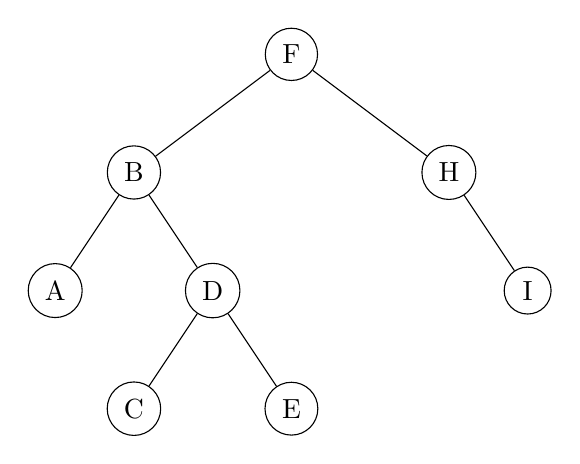
\begin{tikzpicture}[every node/.style={circle,draw},
				level 1/.style={sibling distance=40mm},
				level 2/.style={sibling distance=20mm}]
\node {F}
child { node {B}
	child { node {A} }
	child { node {D}
		child { node {C} }
		child { node {E} } }
}
child { node {H}
	child[missing]
	child { node {I}}};
\end{tikzpicture}
\caption{Boom \ref{fig:BSToef1} na verwijderen van knoop G}
\label{fig:G}
\end{figure}

\begin{figure}[H]
    \centering
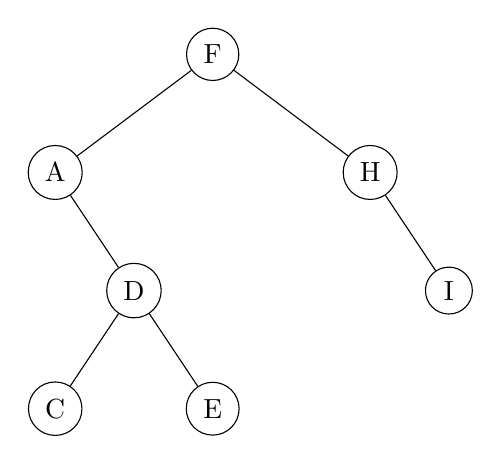
\begin{tikzpicture}[every node/.style={circle,draw},
				level 1/.style={sibling distance=40mm},
				level 2/.style={sibling distance=20mm}]
\node {F}
child { node {A}
	child[missing]
	child { node {D}
		child { node {C} }
		child { node {E} } }
}
child { node {H}
	child[missing]
	child { node {I}}};
\end{tikzpicture}
\caption{Boom \ref{fig:BSToef1} na verwijderen van knoop G en B}
\label{fig:GB}
\end{figure}

\begin{figure}[H]
    \centering
\begin{tikzpicture}[every node/.style={circle,draw},
				level 1/.style={sibling distance=40mm},
				level 2/.style={sibling distance=20mm}]
\node {E}
child { node {A}
	child[missing]
	child { node {D}
		child { node {C} }
		child[missing] }
}
child { node {H}
	child[missing]
	child { node {I}}};
\end{tikzpicture}
\caption{Boom \ref{fig:BSToef1} na verwijderen van knoop G, B en F}
\label{fig:GBF}
\end{figure}


\end{Oplossing}
\begin{Oplossing}{4.1}
De laatste stelling is juist, nl. geen van de vier vorige is correct. Figuur~\ref{fig:tegenvoorbeelden} toont voor elke van deze vier stellingen een tegenvoorbeeld.
\begin{figure}[htbp]
    \centering
    \begin{subfigure}[b]{0.45\textwidth}
        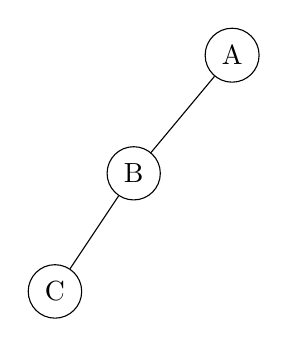
\begin{tikzpicture}[every node/.style={circle,draw},
				level 1/.style={sibling distance=25mm},
				level 2/.style={sibling distance=20mm}]
\node {A}
child { node {B}
	child { node {C} }
	child[missing]
		 }
child[missing]
;
\end{tikzpicture}
        \caption{niet compleet, niet strikt}
        \label{fig:nietcompleetnietstrikt}
    \end{subfigure}
    ~
       \begin{subfigure}[b]{0.45\textwidth}
        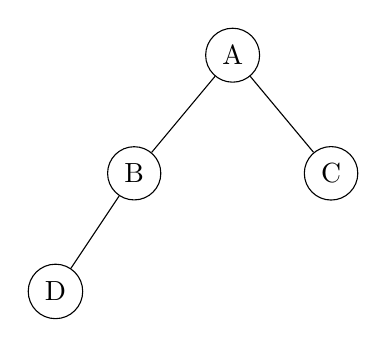
\begin{tikzpicture}[every node/.style={circle,draw},
				level 1/.style={sibling distance=25mm},
				level 2/.style={sibling distance=20mm}]
\node {A}
child { node {B}
	child { node {D} }
	child[missing]
		 }
child { node {C} }
;
\end{tikzpicture}
        \caption{compleet maar niet strikt}
        \label{fig:compleetnietstrikt}
    \end{subfigure}

          \begin{subfigure}[b]{0.45\textwidth}
        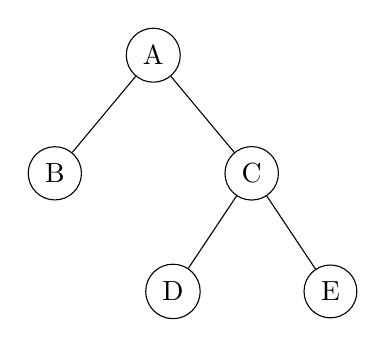
\begin{tikzpicture}[every node/.style={circle,draw},
				level 1/.style={sibling distance=25mm},
				level 2/.style={sibling distance=20mm}]
\node {A}
child { node {B} }
child { node {C}
	child { node {D} }
	child { node {E} }
	}
;
\end{tikzpicture}
        \caption{strikt maar niet compleet}
        \label{fig:striktnietcompleet}
    \end{subfigure}
    ~
    \begin{subfigure}[b]{0.45\textwidth}
        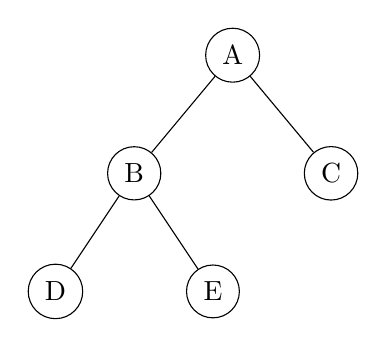
\begin{tikzpicture}[every node/.style={circle,draw},
				level 1/.style={sibling distance=25mm},
				level 2/.style={sibling distance=20mm}]
\node {A}
child { node {B}
	child { node {D} }
	child { node {E} }
	}
child { node {C} }
;
\end{tikzpicture}
        \caption{strikt en compleet}
        \label{fig:striktcompleet}
    \end{subfigure}
    \caption{Tegenvoorbeelden voor de stellingen 1 t.e.m. 4}
    \label{fig:tegenvoorbeelden}
\end{figure}
\end{Oplossing}
\begin{Oplossing}{4.2}
\begin{lstlisting}[caption={count methode}, label=herhoefbbcount]
public int count(E geg) {
	if (geg == null) {
		return 0;
	}
	return (this.data.equals(geg) ? 1 : 0)
			+ (this.leftTree != null ? this.leftTree.count(geg) : 0)
			+ (this.rightTree != null ? this.rightTree.count(geg) : 0);
}
\end{lstlisting}
\end{Oplossing}
\begin{Oplossing}{4.3}
% oplossing: https://www.geeksforgeeks.org/data-structures-binary-search-trees-question-8/
Postorder geeft: 15, 10, 23, 25, 20, 35, 42, 39, 30

Gebruik de preorder wandeling om de gevraagde boom te tekenen.
\end{Oplossing}
\begin{Oplossing}{4.4}
% oplossing: https://www.geeksforgeeks.org/gate-gate-cs-1996-question-52/
Mogelijke oplossingen: nr 1, 3 en 4
\begin{itemize}
\item In nr 2 kan je knoop 60 niet tegenkomen in de zoektocht naar 43 want knoop 60 moet rechts van knoop 50 komen terwijl knoop 43 links moet staan.
\item In nr 5 kan je knoop 18 niet tegenkomen omdat deze knoop links moet staan van knoop 27 terwijl je knoop 43 rechts moet zoeken.
\end{itemize}
\end{Oplossing}
\begin{Oplossing}{4.5}
\begin{lstlisting}[caption={getNodesAtDistance(k) methode}, label=herhoefbbdistance]
public ArrayList<E> getNodesAtDistance(int k) {
	if (k < 0) {
		throw new IllegalArgumentException("Foute waarde voor afstand!");
	}
	ArrayList<E> res = new ArrayList<>();
	if (k == 0) {
		res.add(this.data);
	} else {
		if (this.leftTree != null) {
			res = this.leftTree.getNodesAtDistance(k - 1);
		}
		if (this.rightTree != null) {
			ArrayList<E> rechtsteLijst = this.rightTree.getNodesAtDistance(k - 1);
			res.addAll(rechtsteLijst);
		}
	}
	return res;
}
\end{lstlisting}
\end{Oplossing}
\begin{Oplossing}{4.6}
Je had al door dat dit een andere manier is om de vorige oefening in een opgave te gieten, niet?
\end{Oplossing}
\begin{Oplossing}{4.7}
	\begin{lstlisting}[caption={kinderSom() methode}, label=kinderSom]
	
public class BinaryTreeInt {

private int data;
private BinaryTreeInt leftTree, rightTree;

public BinaryTreeInt(int data) {
	this(data, null, null);
}

public BinaryTreeInt(int data, BinaryTreeInt leftTree, BinaryTreeInt rightTree) {
	this.data = data;
	this.leftTree = leftTree;
	this.rightTree = rightTree;
}
	
public boolean kinderSom() {
	// Controleer of wortel voldoet aan voorwaarden van kindersom
	// Als wortel een blaadje is, voldoet hij
	if (this.isLeaf())
		// bij een blaadje is kinderSom altijd true
		return true;
	// Als wortel geen blaadje is: controle uitvoeren
	else {
		// Bereken som van de waardes van de kinderen
		// De somwaarde van een kind is gelijk aan zijn waarde,
		// tenzij het kind niet bestaat. Dan is de somwaarde gelijk aan 0
		int left_value = (this.leftTree != null ? this.leftTree.data : 0);
		int right_value = (this.rightTree != null ? this.rightTree.data : 0);
		// Als de som niet juist is, voldoet de boom niet aan de voorwaarden
		// Methode kan afgebroken worden
		if (this.data != left_value + right_value)
			return false;
	}
	
	// Als wortel wel voldoet aan voorwaarden, moet de rest van de boom gecontroleerd worden
	return (this.leftTree != null ? this.leftTree.kinderSom() : true) &&
		(this.rightTree != null ? this.rightTree.kinderSom() : true);
}

...
}
	\end{lstlisting}
\end{Oplossing}
\begin{Oplossing}{4.8}

Deze boom kun je bekomen door volgend stappenplan:
\begin{enumerate}
	\item In \emph{post-order} staat de root van de boom altijd achteraan.
	\item Kijk in de \emph{in-order} wandeling waar dat de root zich bevindt. Alles links van de root is de linker sub-boom en alles recht van de root is de rechter sub-boom.
	\item Herhaal deze stappen opnieuw voor de linker en de rechter sub-boom.
\end{enumerate}

Concreet voor deze opgave betekend dit:
\begin{enumerate}
	\item Voor de gehele boom in \emph{post-order} zien we dat ‘D’ achteraan staat en dus de root van onze boom gaat zijn.
	\item De linker subboom bestaat uit ‘FHCA’ \emph{in-order} en de rechter subboom uit ‘EGB’ \emph{in-order}.
	\item De linker subboom in \emph{post-order} bestaat uit ‘FCHA’ en de rechter subboom in \emph{post-order} bestaan uit ‘GEB’.
	\item Voor de linker subboom in \emph{post-order} zien we dat ‘A’ achteraan staat en dus de root van onze subboom gaat zijn.
	\item De linker sub-subboom bestaat uit ‘FHC’ \emph{in-order} en de rechter sub-subboom is leeg.
	\item De linker sub-subboom in \emph{post-order} bestaat uit ‘FCH’ en de rechter sub-subboom is nog steeds leeg.
	\item Voor de linker sub-subboom in \emph{post-order} zien we dat ‘H’ achteraan staat en dus de root van onze volgende subboom gaat zijn.
	\item Blijft dit herhalen tot links en rechts geen subbomen meer hebben.
\end{enumerate}
Figuur~\ref{fig:exjuni19inpost} op pagina~\pageref{fig:exjuni19inpost} toont de boom.
\begin{figure}[htbp]
    \centering
\begin{tikzpicture}[every node/.style={circle,draw},
				level 1/.style={sibling distance=50mm},
				level 2/.style={sibling distance=30mm},
				level 3/.style={sibling distance=20mm}]
\node {D}
child { node {A}
	child { node {H}
		child { node {F} }
		child {node {C} }
	}
	child[missing]
}
child { node {B}
	child { node {E}
		child[missing]
		child { node {G} }	
	}
	child[missing]
};
\end{tikzpicture}
\caption{Binaire boom horend bij de gegeven in en post-order uitvoer}
    \label{fig:exjuni19inpost}
\end{figure}
\end{Oplossing}
\begin{Oplossing}{4.9}
Steun op de eigenschappen van een BST: een binaire boom, met alle knopen links van een knooppunt kleiner dan dit knooppunt en in de rechterboom van het knooppunt allemaal waarden die groter zijn. Je bekomt dan de boom in figuur~\ref{fig:herhoefBST1}. Kijk na dat die inderdaad de gegeven pre-order volgorde geeft. Als je nu op deze BST de post-order wandeling doet bekom als uitvoer: 15, 10, 23, 25, 20, 35, 42, 39, 30.
\begin{figure}[htbp]
    \centering
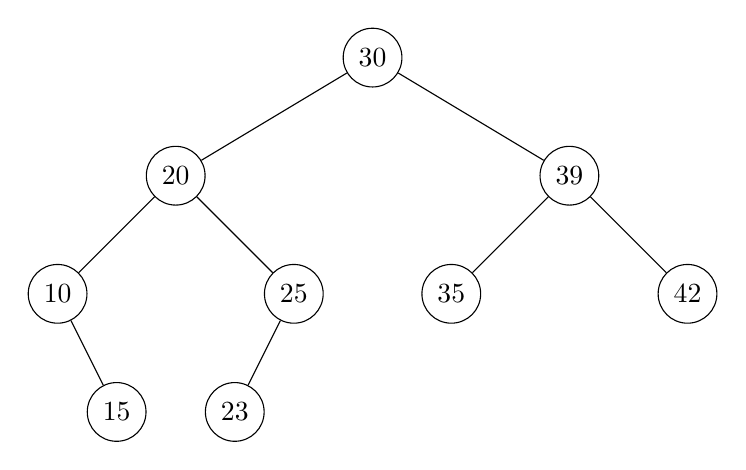
\begin{tikzpicture}[every node/.style={circle,draw},
				level 1/.style={sibling distance=50mm},
				level 2/.style={sibling distance=30mm},
				level 3/.style={sibling distance=15mm}]
\node {30}
child { node {20}
	child { node {10}
		child[missing]
		child {node {15}}
		 }
	child { node {25}
		child { node {23} }
		child[missing]}
}
child { node {39}
	child { node {35}}
	child { node {42}}
};
\end{tikzpicture}
\caption{BST horend bij de gegeven pre-order uitvoer}
    \label{fig:herhoefBST1}
\end{figure}
\end{Oplossing}
\begin{Oplossing}{4.10}
Een goede manier om aan deze oefening te beginnen is een complete binaire boom tekenen met 10 knooppunten (figuur~\ref{fig:herhoefBST2Stap1}).
\begin{figure}[htbp]
    \centering
\begin{tikzpicture}[every node/.style={circle,draw},
				level 1/.style={sibling distance=50mm},
				level 2/.style={sibling distance=25mm},
				level 3/.style={sibling distance=13mm}]
\node {\phantom{7}}
child { node {\phantom{4}}
	child { node {\phantom{2}}
		child { node {\phantom{1}}}
		child {node {\phantom{3}}}
		 }
	child { node {\phantom{6}}
		child { node {\phantom{5}} }
		child[missing]}
}
child { node {\phantom{9}}
	child { node {\phantom{8}}}
	child { node {\phantom{9}}}
};
\end{tikzpicture}
\caption{complete BST voor 10 getallen}
    \label{fig:herhoefBST2Stap1}
\end{figure}
Logisch redeneren met behulp van de basiskenmerken van een BST op deze blanco figuur levert in een aantal stappen de gewenste oplossing. Je kan bvb. volgende info gemakkelijk bekomen:
\begin{itemize}
\item links onderaan moet 1 staan (kleinste getal)
\item rechts onderaan moet 10 staan (grootste getal)
\item er zijn drie getallen groter dan de wortel, dus moet de wortel een 7 zijn
\item …
\end{itemize}
Je bekomt uiteindelijk figuur~\ref{fig:herhoefBST2Stap2}.
\begin{figure}[htbp]
    \centering
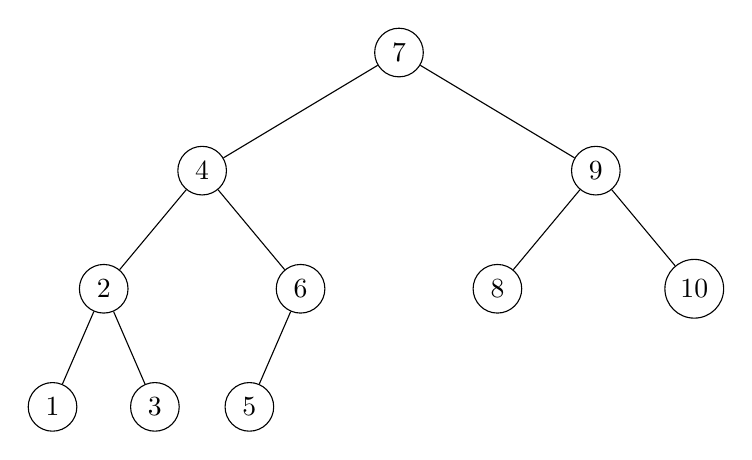
\begin{tikzpicture}[every node/.style={circle,draw},
				level 1/.style={sibling distance=50mm},
				level 2/.style={sibling distance=25mm},
				level 3/.style={sibling distance=13mm}]
\node {7}
child { node {4}
	child { node {2}
		child { node {1}}
		child {node {3}}
		 }
	child { node {6}
		child { node {5} }
		child[missing]}
}
child { node {9}
	child { node {8}}
	child { node {10}}
};
\end{tikzpicture}
\caption{complete BST met getallen van 1 tot 10 ingevuld}
    \label{fig:herhoefBST2Stap2}
\end{figure}
Als je nu “laag per laag” aanvult komt alles waar het hoort te staan. De volgorde wordt dus: 7, 4, 9, 2, 6, 8, 10, 1, 3, 5, of liever gezegd “één van de mogelijke volgordes”. Snap je dat bvb. 7, 9, 4, … ook perfect mogelijk is?

\end{Oplossing}
\begin{Oplossing}{4.11}
De resulterende boom heeft diepte 5 (figuur~\ref{fig:herhoefBST3}).
\begin{figure}[htbp]
    \centering
\begin{tikzpicture}[every node/.style={circle,draw},
				level 1/.style={sibling distance=45mm},
				level 2/.style={sibling distance=25mm},
				level 3/.style={sibling distance=18mm}]
\node {7}
child { node {5}
	child { node {1}
		child { node {0}}
		child {node {3}
			child {node {2}}
			child {node {4}}
			}
		 }
	child { node {6}}
}
child { node {8}
	child[missing]
	child { node {9}}
};
\end{tikzpicture}
\caption{BST als resultaat van invullen in volgorde van 7, 5, 1, 8, 3, 6, 0, 9, 4 en 2}
    \label{fig:herhoefBST3}
\end{figure}
\end{Oplossing}
\begin{Oplossing}{4.12}
De blaadjes van deze boom hebben als datavelden 67 en 83. De boom wordt getoond in figuur~\ref{fig:herhoefBST4}.
\begin{figure}[htbp]
    \centering
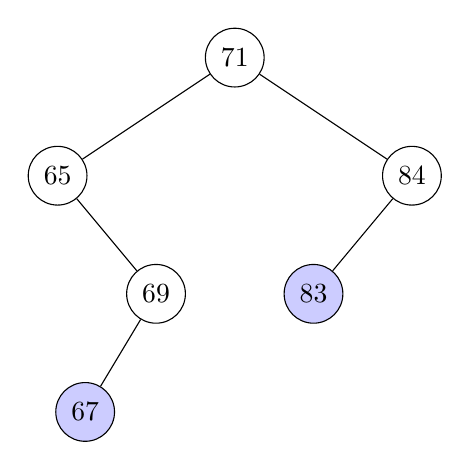
\begin{tikzpicture}[every node/.style={circle,draw},
				level 1/.style={sibling distance=45mm},
				level 2/.style={sibling distance=25mm},
				level 3/.style={sibling distance=18mm}]
\node {71}
child { node {65}
	child[missing]
	child { node {69}
		child {node[fill=blue!20] {67}}
		child[missing]
	}
}
child { node {84}
	child { node[fill=blue!20]  {83}}
	child[missing]
};
\end{tikzpicture}
\caption{BST als resultaat van invullen in volgorde van 71, 65, 84, 69, 67 en 83}
    \label{fig:herhoefBST4}
\end{figure}
\end{Oplossing}
\begin{Oplossing}{4.13}
Pad 9, 85, 47, 68, 43, 57, 55 kan niet omdat $43 < 47$. Maak zelf de figuur, waarbij je telkens links of rechts gaat afhankelijk van of het nieuwe getal kleiner of groter is dan het vorige. Als je ergens naar rechts gaat, moeten alle getallen die daarna komen groter zijn dan dit vorige getal en die voorwaarde wordt hier geschonden.
\end{Oplossing}
\begin{Oplossing}{4.14}
Figuur~\ref{fig:bstex1opl} op pagina~\pageref{fig:bstex1opl} toont de oplossing. In de plaats van het getal 35 mag elk geheel getal tussen 30 en 40 komen (grenzen 30 en 40 niet inbegrepen). Wat het verwijderen van de knoop met waarde 10 betreft: ofwel verdwijnt het blaadje met waarde 9 en komt de waarde in de knoop waar nu 10 staat. Ofwel schuift de knoop 13 eentje op en neemt de plaats in van de waarde 10.
\begin{figure}[htbp]
    \centering
\begin{tikzpicture}[every node/.style={circle,draw},
				level 1/.style={sibling distance=50mm},
				level 2/.style={sibling distance=35mm},
				level 3/.style={sibling distance=20mm},
				level 4/.style={sibling distance=10mm}]
\node {15}
child { node {10}
	child { node {8}
		child { node {4}
			child[missing]
			child { node {6} }
		}
		child { node {9} }
		}
	child { node {13}
		child[missing]
		child { node {14} }
} }
child { node {30}
	child[missing]
	child { node {40}
		child { node {35} }
		child { node {41}}
	}
	};
\end{tikzpicture}

\caption{Gewijzigde BST}
    \label{fig:bstex1opl}
\end{figure}
\end{Oplossing}
\begin{Oplossing}{4.15}
Figuur~\ref{fig:bstex2opl} op pagina~\pageref{fig:bstex2opl} toont de oplossing van de eerste twee vragen. Voor het antwoord op de derde vraag kan ofwel de knoop met waarde L ofwel de knoop met waarde O de plaats innemen van M.
\begin{figure}[htbp]
    \centering
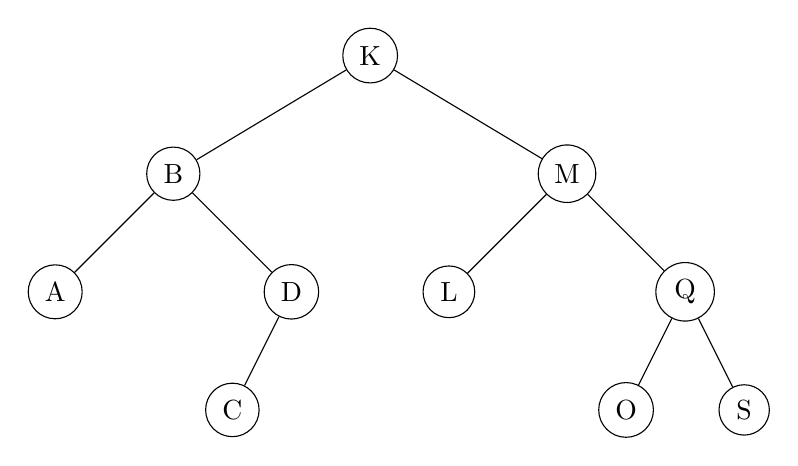
\begin{tikzpicture}[every node/.style={circle,draw},
				level 1/.style={sibling distance=50mm},
				level 2/.style={sibling distance=30mm},
				level 3/.style={sibling distance=15mm}]
\node {K}
child { node {B}
		child { node {A} }
		child { node {D}
			child { node {C} }
			child[missing]
		}
}
child{ node {M}
	child{ node {L} }
	child { node {Q}
		child { node {O} }
		child { node {S}}
	}
};
\end{tikzpicture}
\caption{Gewijzigde BST}
    \label{fig:bstex2opl}
\end{figure}
\end{Oplossing}
\begin{Oplossing}{4.16}

\end{Oplossing}
\begin{Oplossing}{4.17}
De boom in figuur~\ref{fig:aug18opl} op pagina~\pageref{fig:aug18opl} is de gevraagde complete binaire boom. Wat deel twee van de vraag betreft: er zijn vele mogelijke volgordes van getallen. Eén zo'n volgorde is: $5, -3, 3, -4, -8, 9, 6, 10$. Het volstaat om de laatste twee getallen in de andere volgorde te kiezen (dus eerst 10 en dan 6) en je bekomt dezelfde complete BST. Die wordt getoond in figuur~\ref{fig:aug18bopl} op pagina~\pageref{fig:aug18bopl}.
\begin{figure}[htbp]
    \centering
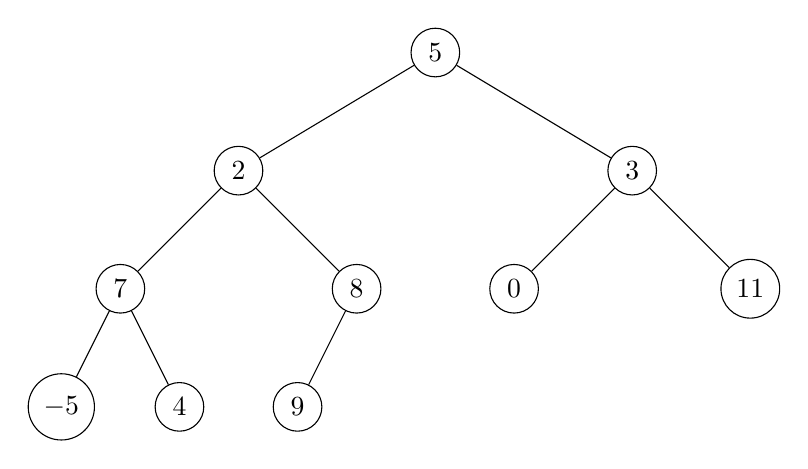
\begin{tikzpicture}[every node/.style={circle,draw},
				level 1/.style={sibling distance=50mm},
				level 2/.style={sibling distance=30mm},
				level 3/.style={sibling distance=15mm}]
\node {5}
child { node {2}
		child { node {7}
			child { node {$-5$} }
			child { node {4} }
		}
		child { node {8}
			child { node {9} }
			child[missing]
		}
}
child{ node {3}
	child{ node {0} }
	child { node {11} }
};
\end{tikzpicture}
\caption{Oplossing voor de complete binaire boom}
    \label{fig:aug18opl}
\end{figure}
\begin{figure}[htbp]
    \centering
\begin{tikzpicture}[every node/.style={circle,draw},
				level 1/.style={sibling distance=50mm},
				level 2/.style={sibling distance=30mm},
				level 3/.style={sibling distance=15mm}]
\node {5}
child { node {$-3$}
		child { node {$-4$}
			child { node {$-8$} }
			child[missing]
		}
		child { node {3} }
}
child{ node {9}
	child{ node {6} }
	child { node {10} }
};
\end{tikzpicture}
\caption{Deze complete BST bekom je}
    \label{fig:aug18bopl}
\end{figure}
\end{Oplossing}
\begin{Oplossing}{4.18}
Figuur~\ref{fig:bstexjuni19opl} op pagina~\pageref{fig:bstexjuni19opl} toont de BST.
\begin{figure}[htbp]
    \centering
\begin{tikzpicture}[every node/.style={circle,draw},
				level 1/.style={sibling distance=70mm},
				level 2/.style={sibling distance=50mm},
				level 3/.style={sibling distance=30mm},
				level 4/.style={sibling distance=20mm}]
\node {T}
child { node {L}
	child { node {D}
		child { node {B}
			child {node {A} }
			child {node {C} }
			}
		child { node {E} }
		}
	child { node {M}
		child[missing]
		child { node {S} }
} }
child { node {V}
	child[missing]
	child[missing]
	};
\end{tikzpicture}
\caption{BST voor studentendossiers}
    \label{fig:bstexjuni19opl}
\end{figure}
Er zijn vele volgordes mogelijk om deze BST te construeren. Zo kan je laag per laag werken, of er voor kiezen om eerst de linkerboom af te werken en dan de rechter (of omgekeerd). Eén van vele mogelijk volgordes is: T, L, V, D, B, E, A, C, M, S. Het volstaat bvb. om de L en de V van plaats te verwisselen om een andere goede volgorde te bekomen. In arrayvoorstelling geeft dit het volgende (we stellen een lege cel voor door het symbool *): [T, L, V, D, M, *, *, B, E, *, S, *, *, *, *, A, C].

Om deze 10 dossiers voor te stellen in een heap zijn er vele mogelijkheden. Figuur~\ref{fig:bstexjuni19oplheap} op pagina~\pageref{fig:bstexjuni19oplheap} toont er eentje. Om diepte 13 te bereiken moet je veel nodes toevoegen, want de boom moet compleet zijn. Op elk niveau staat een ‘macht van 2’ aantal getallen. Op diepte 4 moeten er $2^3$ knopen zijn. Er staan er al drie, dus je voegt er nog $2^3 - 3$ toe. Op de volgende dieptes voeg je $2^4 + 2^5 + \cdots + 2^{11}$ knopen toe. Tenslotte op diepte 13 nog 1 knoop. We berekenen dus volgende som:
\[
2^3 - 3 + 2^4 + 2^5 + 2^6 + \cdots + 2^{10} + 2^{11} + 1 = 4086
\]
\begin{figure}[htbp]
    \centering
\begin{tikzpicture}[every node/.style={circle,draw},
				level 1/.style={sibling distance=70mm},
				level 2/.style={sibling distance=50mm},
				level 3/.style={sibling distance=30mm},
				level 4/.style={sibling distance=20mm}]
\node {V}
child { node {L}
	child { node {D}
		child { node {A} }
		child { node {B} }
	}
	child { node {E}
		child { node {C} }
		child[missing]
	}
}
child { node {T}
	child { node {M} }
	child { node {S} }
};
\end{tikzpicture}
\caption{Max-heap voor studentendossiers}
    \label{fig:bstexjuni19oplheap}
\end{figure}
\end{Oplossing}
\begin{Oplossing}{4.19}
\begin{enumerate}
\item “kat de krollen de krabt . van trap de”
\item Figuur~\ref{fig:dansendemuizen} op pagina~\pageref{fig:dansendemuizen} toont de complete binaire boom.
\begin{figure}[htbp]
    \centering
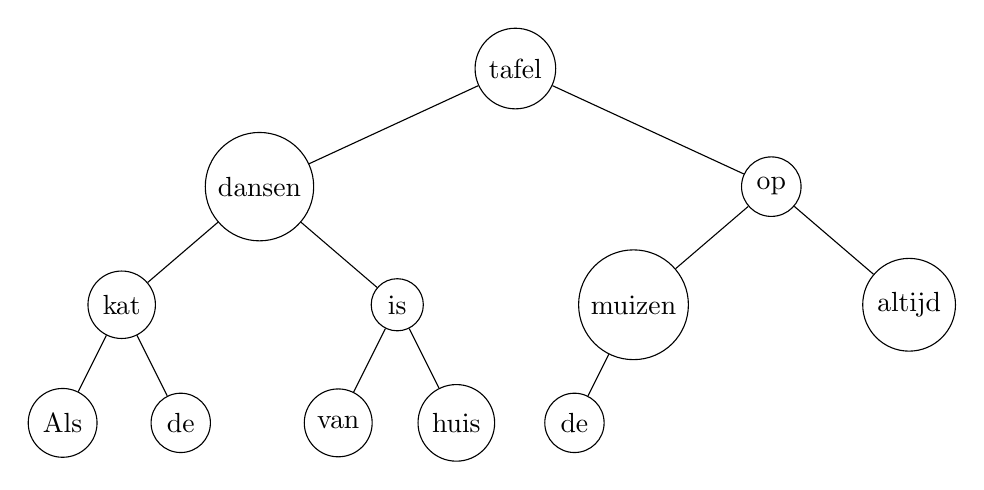
\begin{tikzpicture}[every node/.style={circle,draw},
				level 1/.style={sibling distance=65mm},
				level 2/.style={sibling distance=35mm},
				level 3/.style={sibling distance=15mm},
				level 4/.style={sibling distance=10mm}]
\node {tafel}
child { node {dansen}
	child { node {kat}
		child { node {Als} }
		child { node {de} }
	}
	child { node {is}
		child { node {van} }
		child { node {huis}	}
	}
}
child { node {op}
	child { node {muizen}
		child { node {de} }
		child[missing]
	}
	child { node {altijd} }
};
\end{tikzpicture}
\caption{Als de kat van huis is dansen de muizen altijd op tafel}
    \label{fig:dansendemuizen}
\end{figure}
\end{enumerate}
\end{Oplossing}
\begin{Oplossing}{4.20}
\begin{lstlisting}
   public BinaryTree<E> deelZonder(E wortelInfo) {
        if (wortelInfo == null || !this.contains(wortelInfo))
            return null;
        // wortelInfo == data, dus hele boom verwijderen
        if (this.data == wortelInfo) {
            return null;
        }
        // wortelInfo = linkerkind van data, dus hele linkertak verwijderen
        if (this.leftTree!=null && this.leftTree.data.equals(wortelInfo)){
            return new BinaryTree(this.data,null,this.rightTree);
        }
        // wortelInfo == rechterkind van data, dus hele rechtertak verwijderen
        if (this.rightTree!= null && this.rightTree.equals(wortelInfo)){
            return new BinaryTree(this.data,this.rightTree,null);
        }
        BinaryTree newLeftTree, newRightTree;
        // als wortelInfo in linkertak zit: nieuwe linkertak maken zonder wortelInfo
        if (this.leftTree != null && this.leftTree.contains(wortelInfo))
            newLeftTree = this.leftTree.deelZonder(wortelInfo);
        // anders linkertak behouden
        else newLeftTree = this.leftTree;
        // idem voor rechtertak
        if (this.rightTree!=null && this.rightTree.contains(wortelInfo))
            newRightTree = this.rightTree.deelZonder(wortelInfo);
        else
            newRightTree = this.rightTree;
        // resulterende boom terug samenstellen
        return new BinaryTree<>(this.data,newLeftTree,newRightTree);
    }
\end{lstlisting}
\end{Oplossing}
\begin{Oplossing}{4.21}
\begin{lstlisting}
   public boolean isStrict() {
        // wortel == blaadje
        if (this.isLeaf())
            return true;
        // wortel heeft linker- en rechtertak, dus rest van boom controleren
        if ((this.leftTree != null && this.rightTree != null)) {
            return this.leftTree.isStrict() && this.rightTree.isStrict();
        }
        // bij wortel ontbreekt linker- of rechtertak
        return false;

    }
    \end{lstlisting}
\end{Oplossing}
\begin{Oplossing}{4.22}
Werkwijze: Bekijk de code van de methode \verb/printInOrder()/. In die methode schrijf je eerst recursief de waarden uit van de linkerboom, dan de waarde van de wortel, dan behandel je de rechterboom. Hier kan je ook zo te werk gaan. De waarden zullen dan van klein naar groot geordend zijn.

In tegenstelling tot \verb/printInOrder()/ schrijven we de waarden nu niet uit naar de console, maar verzamelen we ze in een lijst. Dat is gelijkend op hetgeen je deed in de methode \verb/getDataLeaves()/.

Tenslotte hoef je niet steeds te zoeken over het volledige interval. Immers, in een BST zijn de elementen links van wortel kleiner dan wortel en rechts ervan groter. Je kan het interval waarin je zoekt dus steeds kleiner maken.

\begin{lstlisting}
public class BinarySearchTree<E extends Comparable<E>> {
    private BinaryTree<E> root;

   ...

       public List<E> geefKnopenBinnenInterval(E min, E max) {
        if (this.isEmpty())
            throw new IllegalStateException("Empty tree");
        return this.root.geefKnopenBinnenInterval(min, max);
    }

    private class BinaryTree<E extends Comparable<E>> {
        private E data;
        private BinaryTree<E> leftTree, rightTree;

	...
	
	        public List<E> geefKnopenBinnenInterval(E min, E max) {
            if (min == null || max == null)
                throw new IllegalArgumentException("Geen effectief interval");
            List<E> result = new ArrayList<>();
            if (min.compareTo(max) > 0)
                return result;

                // zoek eerst waarden in linkerboom
                // je hoeft niet over volledig interval te zoeken
                // want alle knopen in linkerboom zijn kleiner dan wortel
            if (this.leftTree != null)
                result.addAll(this.leftTree.geefKnopenBinnenInterval(min, getMinimum(this.data, max)));
                // controleer of data in gevraagde interval zit
            if (this.data.compareTo(min) >= 0 && this.data.compareTo(max) <= 0)
                result.add(this.data);
                // behandel rechterboom
            if (this.rightTree != null)
                result.addAll(this.rightTree.geefKnopenBinnenInterval(getMaximum(min, this.data), max));
            return result;
        }

        private E getMinimum(E object1, E object2) {
            if (object1.compareTo(object2) <= 0)
                return object1;
            else
                return object2;
        }

        private E getMaximum(E object1, E object2) {
            if (object1.compareTo(object2) >= 0)
                return object1;
            else
                return object2;
        }
    }
\end{lstlisting}
\end{Oplossing}
\begin{Oplossing}{5.1}
Zoals we in de theorie zagen, moet je een bepaalde waarde afspreken om aan te geven dat een bepaald kind ontbreekt. Laten we dat voor de eenvoud hier gewoon voorstellen door het getal \verb+0+.
Een mogelijke arrayimplementatie voor figuur~\ref{fig:arrayimpl1} is:\\
\verb+[F, B, G, A, D, 0, I, 0, 0, C, E, 0, 0, H]+ \\
Voor figuur~\ref{fig:arrayimpl2}: \verb+[3, 2, 5, 1, 4]+. Aangezien dit een complete binaire boom is, bevat de array geen “nullen”.
\end{Oplossing}
\begin{Oplossing}{5.2}
Een goed startpunt om deze oefening op te lossen is een tekening maken. Het lukt natuurlijk niet om heel de boom te tekenen, maar we kunnen wel de eerste niveau's tekenen en dan de kracht van abstractie toepassen op zoek naar een patroon.

Bekijk figuur~\ref{fig:1000knopen}. Op niveau 1 is er één knoop met nummer 0. Op niveau 2 zijn er twee knopen, nummer 1 en 2. Als we deze getallen in een tabel zetten (tabel~\ref{tbl:1000knopen}) valt er één en ander op.
\begin{figure}[htbp]
    \centering
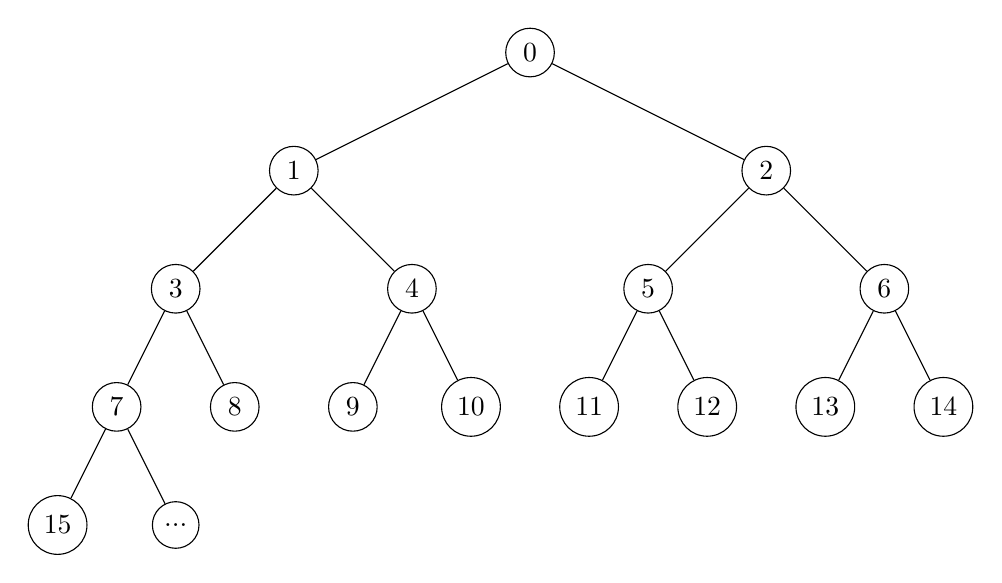
\begin{tikzpicture}[every node/.style={circle,draw},
				level 1/.style={sibling distance=60mm},
				level 2/.style={sibling distance=30mm},
				level 3/.style={sibling distance=15mm}]
\node {0}
child { node {1}
	child { node {3}
		child { node {7}
			child {node {15}}
			child {node {...}}
		}
		child { node {8} }
	 }
	child { node {4}
		child { node {9} }
		child { node {10} }
		}
}
child { node {2}
	child { node {5}
		child { node {11} }
		child { node {12} }
	 }
	child { node {6}
		child { node {13} }
		child { node {14} }
	}
};
\end{tikzpicture}
\caption{Op weg naar 1000 knooppunten, genummerd van 0 tot 999}
    \label{fig:1000knopen}
\end{figure}

\begin{table}[ht]
  \centering
  \caption{Overzicht van alle knopen}
  \begin{tabular}{rrrr}
    \toprule
niveau & aantal & nummers & totaal \\
\midrule
1 & 1 & 0 & 1\\
2 & 2 & $1 \rightarrow 2$ & 3\\
3 & 4 & $3 \rightarrow 6$ & 7\\
4 & 8 & $7 \rightarrow 14$ & 15\\
5 & 16 & $15 \rightarrow 30$ & 31\\
... & ... & ... & ...\\
$i$ & $2^{i-1}$ & $2^{i-1}-1 \rightarrow 2^i-2$ & $2^i - 1$\\
... & ... & ... & ...\\
9 & 256 & $255 \rightarrow 510$ & 511\\
\bottomrule
  \end{tabular}
  \label{tbl:1000knopen}
\end{table}
Op niveau 9 zijn er dus 256 knooppunten, genummerd van 255 tot 510. In totaal heeft deze binaire boom op de eerste 9 niveau's samen 511 elementen. Op niveau 10 zou er plaats zijn voor 512 elementen, maar dat hoeft niet meer. Als er in totaal 1000 knooppunten moeten zijn, zal het laagste niveau nog $1000-511=489$ knopen tellen.

Met deze informatie kunnen we nu de vragen beantwoorden:
\begin{oefenumerate}
	\item \emph{Waar vind je de ouder van de knoop die zich in de array op index 256 bevindt?} De knoop met nummer 256 staat op niveau 9 als tweede van links. Het is het rechterkind van de knoop op niveau 8 met nummer 127. Dat is de eerste knoop links op het achtste niveau.
	\item \emph{Waar vind je de rechterbuur (op hetzelfde niveau) van de knoop die zich in de array op index 72 bevindt?} Knoop 72 bevindt zich op niveau 7, meerbepaald de tiende knoop op dit niveau. De rechterbuur van 72 is natuurlijk knoop 73. Beide knopen hebben een verschillende ouder (welke?).
	\item \emph{Heeft de knoop die zich in de array op index 249 bevindt kleinkinderen?} De kinderen van knoop $i$ zijn knopen $2i+1$ en $2i+2$. Knoop 249 heeft dus twee kinderen: 499 en 500. De kinderen van 499 zijn nummer 999 en 1000, die van 500 zijn 1001 en 1002. Vermits deze boom maar duizend knopen heeft, heeft de laatste knoop het nummer 999. Daaruit volgt dat knoop 249 wel degelijk één kleinkind heeft, nl. de allerlaatste knoop op het tiende niveau rechts, met nummer 999.
\end{oefenumerate}
\end{Oplossing}
\begin{Oplossing}{5.3}
\begin{lstlisting}[caption={kleinste waarde van min-heap}, label=minheapkleinste]
public E getMin() {
	if (this.values.size() == 0) {
		throw new IllegalStateException();
	} else {
		return this.values.get(0);
	}
}
\end{lstlisting}

\end{Oplossing}
\begin{Oplossing}{5.4}
\begin{lstlisting}[caption={bubbleUp methode}, label=minheapbubbleUp]
private void bubbleUp() {
	int index = this.values.size() - 1; //start met laatste element
		
	while (heeftOuder(index) && ouder(index).compareTo(values.get(index)) > 0) {
		//ouder en kind staan in verkeerde volgorde, wissel ze om
		this.wisselOm(index, ouderIndex(index));
		index = ouderIndex(index);
	}
}

private boolean heeftOuder(int i) {
	return i >= 1;
}

private E ouder(int i) {
	return values.get(ouderIndex(i));
}

private int ouderIndex(int i) {
	return (i - 1)/2;
}
	
private void wisselOm(int i, int j) {
	//wissel i-de en j-de element in de ArrayList om
	E hulp = this.values.get(i);
	this.values.set(i, this.values.get(j));
	this.values.set(j, hulp);
}
\end{lstlisting}
\end{Oplossing}
\begin{Oplossing}{5.5}
\begin{lstlisting}[caption={bubbleDown methode}, label=minheapbubbleDown]
private void bubbleDown() {
	int index = 0; //start met de wortel
		
	boolean wisselOK = true;
	while (heeftLinkerKind(index) && wisselOK) {
		//welk kind is het kleinste?
		int indexKleinsteKind = indexLinkerKind(index);
		if (heeftRechterKind(index)
			&& values.get(indexKleinsteKind).compareTo(values.get(indexRechterKind(index))) > 0) {
			indexKleinsteKind = indexRechterKind(index);
		}
		//vergelijk ouderwaarde met waarde van kleinste kind
		if (values.get(index).compareTo(values.get(indexKleinsteKind)) > 0) {
			//foute volgorde, wissel om				
			this.wisselOm(index, indexKleinsteKind);
		} else {
			//volgorde OK, while lus mag stoppen
			wisselOK = false;
		}
			
		//vertrek nu vanuit de index van het kleinste kind
		index = indexKleinsteKind;
	}
}

private int indexLinkerKind(int i) {
	return 2 * i + 1;
}
	
private int indexRechterKind(int i) {
	return 2 * i + 2;
}
	
private boolean heeftLinkerKind(int i) {
	return indexLinkerKind(i) < values.size();
}
	
private boolean heeftRechterKind(int i) {
	return indexRechterKind(i) < values.size();
}
\end{lstlisting}

\end{Oplossing}
\begin{Oplossing}{5.6}
\begin{lstlisting}[caption={getPath methode}, label=minheapgetPath]
public ArrayList<E> getPath(E value) {
	int index = this.values.indexOf(value);
	if (index == -1) {
		//value komt niet voor in de heap
		return null;
	} else {
		//value zit in heap, index = plaats van eerste voorkomen
		ArrayList<E> pad = new ArrayList<>();
		pad.add(value);
		while (index > 0) {
			//we zijn nog niet aan de wortel
			index = (index - 1)/2; //ouder
			pad.add(0, this.values.get(index)); //voeg vooraan toe
		}
	return pad;	
	}
}
\end{lstlisting}
\end{Oplossing}
\begin{Oplossing}{6.1}
Het volstaat om de getallen in een boom te zetten en te kijken of de max-heap eigenschap gerespecteerd is. Het juiste antwoord is b), maar wel zullen bij wijze van uitleg laten zien waarom antwoord a) niet correct is. Zet de zeven getallen in volgorde in een complete binaire boom. Je bekomt figuur~\ref{fig:foutemaxheap}. Voor een max-heap moet elke ouder groter zijn dan zijn eventuele kinderen. Aan deze eis is niet voldaan door de knopen met de getallen 12 en 13.
\begin{figure}[htbp]
    \centering
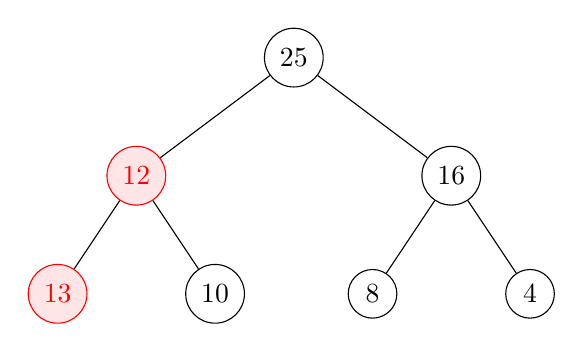
\begin{tikzpicture}[every node/.style={circle,draw},
				level 1/.style={sibling distance=40mm},
				level 2/.style={sibling distance=20mm}]
\node {25}
child { node[red, fill=red!10] {12}
	child { node[red, fill=red!10] {13} }
	child { node {10}}
}
child { node {16}
	child { node {8}}
	child { node {4}}
};
\end{tikzpicture}
\caption{Foute max-heap uit a)}
    \label{fig:foutemaxheap}
\end{figure}
\end{Oplossing}
\begin{Oplossing}{6.2}
Voeg alle elementen element per element toe, gevolgd door een eventuele “bubble up”. Je bekomt figuur~\ref{fig:maxheapbubbleup} en dus antwoord a).
\begin{figure}[htbp]
    \centering
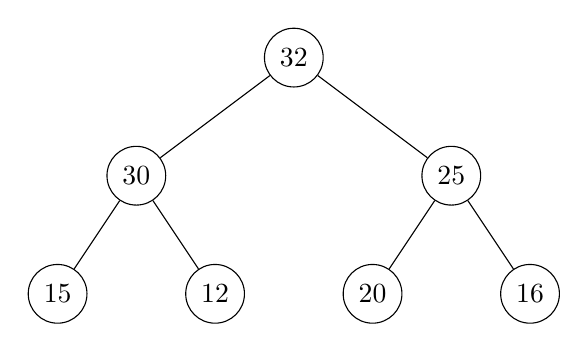
\begin{tikzpicture}[every node/.style={circle,draw},
				level 1/.style={sibling distance=40mm},
				level 2/.style={sibling distance=20mm}]
\node {32}
child { node {30}
	child { node {15} }
	child { node {12}}
}
child { node {25}
	child { node {20}}
	child { node {16}}
};
\end{tikzpicture}
\caption{Max-heap met de getallen 32, 15, 20, 30, 12, 25 en 16 in die volgorde toegevoegd}
    \label{fig:maxheapbubbleup}
\end{figure}
\end{Oplossing}
\begin{Oplossing}{6.3}
Diepte 9.

In een binaire min-heap van 1023 elementen zijn 10 lagen. Daarom kan je de getallen 2 tot en met 9 telkens als linkerkind van het vorige toevoegen.
\end{Oplossing}
\begin{Oplossing}{6.4}
%opl: https://www.geeksforgeeks.org/gate-gate-cs-2014-set-2-question-22/
Figuur~\ref{fig:levelorderheap} toont de originele boom plus de toevoeging van de getallen 1 en 7. Het getal 1 wordt gewoon het linkerkind van 5, 7 wordt het rechterkind met als gevolg dat de 7 ‘naar boven opborrelt’ en dus gewisseld wordt met 5. De level-order output wordt dan: 10, 8, 7, 3, 2, 1, 5.
\begin{figure}[htbp]
    \centering
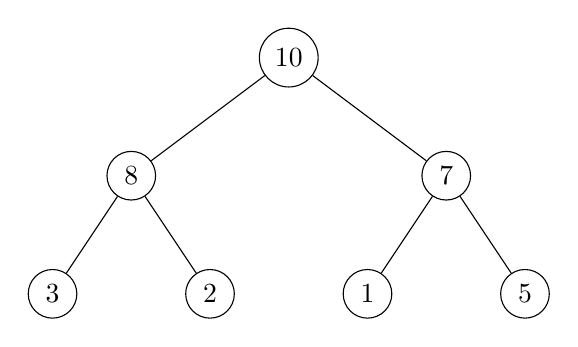
\begin{tikzpicture}[every node/.style={circle,draw},
				level 1/.style={sibling distance=40mm},
				level 2/.style={sibling distance=20mm}]
\node {10}
child { node {8}
	child { node {3}}
	child { node {2}}
}
child { node {7}
	child { node {1}}
	child { node {5}}
};
\end{tikzpicture}
\caption{Max heap die bewandelt wordt in ‘level order’}
\label{fig:levelorderheap}
\end{figure}
\end{Oplossing}
\begin{Oplossing}{6.5}
\begin{itemize}
\item een binaire min-heap: vliegtuig met minste brandstof moet eerst van de hoop gehaald kunnen worden
\item \verb/[125,840,340,1225,996,780,355]/

\begin{figure}[htbp]
    \centering
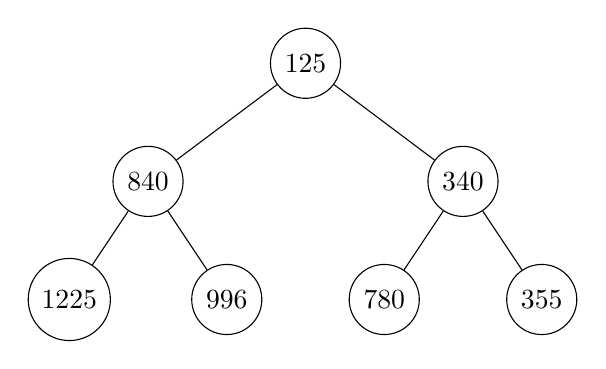
\begin{tikzpicture}[every node/.style={circle,draw},
				level 1/.style={sibling distance=40mm},
				level 2/.style={sibling distance=20mm}]
\node {125}
child { node {840}
	child { node {1225}}
	child { node {996}}
}
child { node {340}
	child { node {780}}
	child { node {355}}
};
\end{tikzpicture}
\caption{Min-heap van vliegtuigen}
\end{figure}
\item \verb/[780, 840, 996, 1225]/
\end{itemize}
\end{Oplossing}
\begin{Oplossing}{6.6}
\begin{enumerate}
\item Op diepte 1 staat er 1 element, op diepte 2 zijn er 2, op diepte 3 zijn er 4. Op diepte 4 staan er 8. Dat zijn dus allemaal machten van 2. Reken na dat er op diepte $i$ juist $2^{i-1}$ getallen kunnen staan. Laten we nu even het \emph{cumulatieve aantal} getallen bekijken, d.w.z. het aantal getallen op een diepte gelijk aan het gegeven getal of een hoger niveau (met lagere diepte). Als voorbeeld: op diepte 4 en alle dieptes erboven (3 2, 1) staan er in totaal 15 elementen. Kijk zelf na dat het hier telkens gaat over 1 minder dan een macht van 2. Het aantal mogelijke getallen op een diepte i of hoger is dus gelijk aan $2^i - 1$. Als $i=9$ als voorbeeld kan je berekenen dat op dit niveau en alle niveau's erboven samen $2^9 - 1 = 511$ getallen kunnen staan. Van 9999 naar 1 zijn in totaal 10000 getallen. Als $i=13$ komen we aan een cumulatief aantal getallen van $2^{13}-1=8191$, wat kleiner is dan 10000. Het getal 1 staat dus op diepte 14.

\item Het feit dat een binaire max-heap compleet is: er zijn dus geen “lege plaatsen” in de array

\item Op index 0 staat het getal 9999, op index 1 het getal 9998 enz. Je merkt dat de som van de index en het getal zelf altijd 9999 is. Dat wil dus zeggen dat het getal 1000 in de array op index $9999-1000=8999$ staat.

\item Het ouderelement van het element 1000 dat op index 8999 staat is $\frac{8999-1}{2}$ afgerond naar beneden, dus index 4499. De waarde van het element op deze index van de array is dus $9999-4499=5500$.

\item De twee kinderen van het element met waarde 1000 (op index 8999) zijn de getallen op indices $8999\cdot 2 + 1$ en $8999\cdot 2 + 2$. Vermits de array maar tot index 9999 gaat, heeft de knoop met waarde 1000 geen kinderen in dit schema.
\end{enumerate}
\end{Oplossing}
\begin{Oplossing}{6.7}
\begin{enumerate}
\item \verb/0,2,6,14,30,61,124/
\item \verb/89,90,179,180,181,182,359/ (de 360ste knoop heeft index 359)
\item neen, want de laatste knoop is kleiner dan zijn ouder  (zie figuur \ref{fig:geenMinHeap} op pg~\pageref{fig:geenMinHeap})
\begin{figure}[htbp]
    \centering
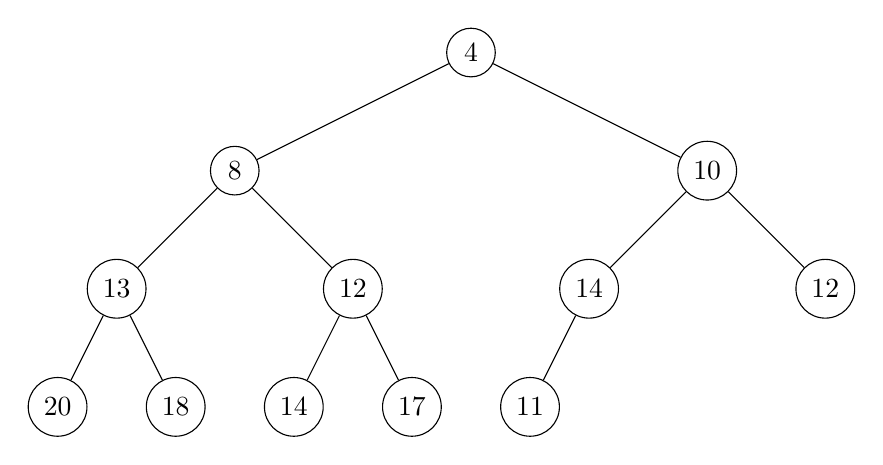
\begin{tikzpicture}[every node/.style={circle,draw},
				level 1/.style={sibling distance=60mm},
				level 2/.style={sibling distance=30mm},
				level 3/.style={sibling distance=15mm}]
\node {4}
child { node {8}
	child { node {13}
		child { node {20} }
		child { node {18}}}
	child { node {12}
		child { node {14} }
		child { node {17}}}
}
child { node {10}
	child { node {14}
		child { node {11} }
		child[missing]}
	child { node {12}}
};
\end{tikzpicture}
\caption{Oplossing bij oefening 2 van \ref{oef:getallen} - geen min-heap}
\label{fig:geenMinHeap}
\end{figure}
\item \verb/[8,13,12,20,18,14,17]/: is wel een min-heap (zie figuur \ref{fig:welMinHeap})
\begin{figure}[htbp]
    \centering
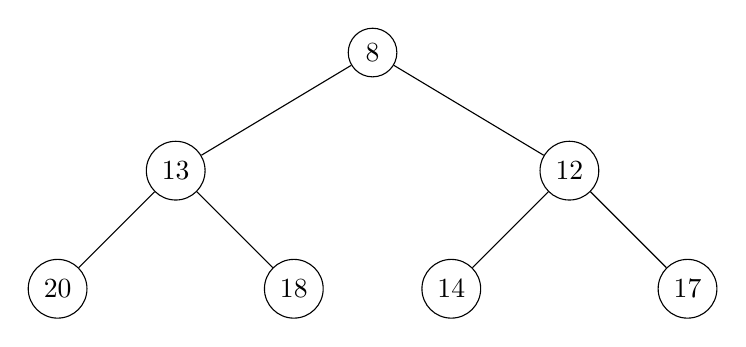
\begin{tikzpicture}[every node/.style={circle,draw},
				level 1/.style={sibling distance=50mm},
				level 2/.style={sibling distance=30mm},
				level 3/.style={sibling distance=15mm}]
\node {8}
	child { node {13}
		child { node {20} }
		child { node {18}}}
	child { node {12}
		child { node {14} }
		child { node {17}}};
\end{tikzpicture}
\caption{Oplossing bij oefening 3 van \ref{oef:getallen} - wel min-heap}
\label{fig:welMinHeap}
\end{figure}
\end{enumerate}
\end{Oplossing}
\begin{Oplossing}{7.1}
$1\rightarrow2\rightarrow5\rightarrow8$ of $1\rightarrow4\rightarrow7\rightarrow8$
\end{Oplossing}
\begin{Oplossing}{7.2}
\begin{enumerate}
\item Een verbindingsmatrix is correct indien
\begin{itemize}
\item het aantal rijen gelijk is aan het aantal kolommen
\item de diagonaal van linksboven naar rechtsonder overal nul is
\item alle elementen gelijk zijn aan $0$ of $1$
\end{itemize}
\item De waarden van de verbindingsmatrix kunnen slechts gelijk zijn aan $0$ en $1$. Het vraagt minder geheugenruimte en het werkt efficiënter als de elementen als een boolean voorgesteld worden.
\end{enumerate}
\end{Oplossing}
\begin{Oplossing}{7.3}
\begin{lstlisting}[caption={findAncestors(int,int)}, label=BFSAncestors]
private boolean rechtstreekseVerbinding(int van, int tot) {
	//System.out.println("verbinding van "+van+" tot "+tot+"?");
	return this.getVerbindingsMatrix()[van - 1][tot - 1];
}

private int[] findAncestors(int start, int destination) {
	int aantalKnopen = this.getAantalKnopen();
	int[] ancestors = new int[aantalKnopen];
	initArray(ancestors, infty);

	Queue<Integer> queue = new LinkedList<>();
	queue.add(start);
	ancestors[start - 1] = 0;

	int huidig = queue.remove();
	while (huidig != destination) {
		//System.out.println("huidig = "+huidig);
		//zoek alle nog niet bezochte knooppunten vanuit huidig
		for (int i = 1; i <= aantalKnopen; i++) {
			if (rechtstreekseVerbinding(huidig, i) && (ancestors[i - 1] == infty)) {
				//System.out.println("ja");
				//voeg knoop i toe aan queue
				queue.add(i);
					
				//duid aan dat huidig de ouder is van i in ancestormatrix
				ancestors[i - 1] = huidig;
			}
		}
		//voorste element van queue wordt nieuwe huidige knoop
		if (!queue.isEmpty()) {
			huidig = queue.remove(); //of .poll() wat geen exception gooit
		} else {
			//queue is leeg, stop maar
			break;
		}
		
	}
	return ancestors;
}

public boolean[][] getVerbindingsMatrix() {
	return verbindingsMatrix;
}


private void initArray(int[] array, int value) {
	for (int i = 0; i < array.length; i++)
		array[i] = value;
}
\end{lstlisting}
\end{Oplossing}
\begin{Oplossing}{7.4}
\begin{lstlisting}[caption={findPath}, label=BFSfindPath]
public List<Integer> findPath(int start, int destination) {
	if (start <= 0 || start > this.getAantalKnopen() || destination <= 0 ||
				destination > this.getAantalKnopen())
		throw new IllegalArgumentException();

	int[] ancestors = this.findAncestors(start, destination);
	List<Integer> path = new LinkedList<>();

	int ouder = ancestors[destination - 1];
	while (ouder != 0 && ouder != infty) {
		path.add(0, destination);;
		destination = ouder;
		ouder = ancestors[destination - 1];
	}
	if (ouder == 0) {
		path.add(0,destination);
	}
	return path;
}
	\end{lstlisting}
\end{Oplossing}
\begin{Oplossing}{8.1}
Gewichtenmatrix $D^{(6)}$ en bijhorende pointermatrix $P$:
\begin{equation*}
D^{(6)}=\begin{bmatrix}
0 & 6 & 3 & 7 & 4 & 6\\
2 & 0 & 5 & 9 & 6 & 8\\
5 & 3 & 0 & 4 & 1 & 3\\
\infty & \infty & \infty & 0 & \infty & 6 \\
5 & 11 & 8 & 3 & 0 & 2\\
\infty & \infty & \infty & 1 & \infty & 0
\end{bmatrix}
\qquad
P=\begin{bmatrix}
0 & 3 & 0 & 6 & 3 & 5 \\
0 & 0 & 1 & 6 & 3 & 5\\
2 &0 &0 & 6 & 0 & 5\\
0 & 0 & 0 & 0 & 0 & 0 \\
0 &  3 & 1 & 6 & 0 & 0 \\
0 & 0 & 0 & 0 & 0 & 0
\end{bmatrix}
\end{equation*}
Enkele paden: $2\rightarrow1\rightarrow3\rightarrow5\rightarrow6$ met lengte 8; $5 \rightarrow 1 \rightarrow 3 \rightarrow  2\rightarrow 4$ met lengte 3
\end{Oplossing}
\begin{Oplossing}{8.2}
\begin{lstlisting}[caption={getPointerMatrix}, label=FloydgetPointerMatrix]
public int[][] getPointerMatrix() {
	int aantal = this.gewichtenMatrix.length;
	int[][] P = new int[aantal][aantal];
	//double[][] D = this.gewichtenMatrix.clone(); fout = shallow clone
	//http://stackoverflow.com/questions/9106131/how-to-clone-a-multidimensional-array-in-java
	//of manuele versie in de nieuwe opgave op toledo
	//argument voor deze clone: is gezien in OOP
	double[][] D = this.gewichtenMatrix.clone();
	for (int i = 0; i < D.length; i++) {
	    D[i] = D[i].clone();
	}

	for (int k = 0; k < aantal; k++) {
		for (int i = 0; i < aantal; i++) {
			for (int j = 0; j < aantal; j++) {
				if (D[i][k] + D[k][j] < D[i][j]) {
					D[i][j] = D[i][k] + D[k][j];
					P[i][j] = k + 1;
				}
			}
		}
	}
	return P;
}
\end{lstlisting}
\end{Oplossing}
\begin{Oplossing}{8.3}
\begin{lstlisting}[caption={getShortestPath}, label=FloydgetShortestPath]
public List<Integer> getShortestPath(int van, int tot, int[][] P) {
	List<Integer> pad = new ArrayList<>();
	if (van == tot) {
		return pad;
	} else {
		int via = P[van - 1][tot - 1];
		if (via == 0){
			pad.add(van);
			pad.add(tot);
		} else {
			pad = getShortestPath(van, via, P);
			pad.remove(pad.size() - 1); //anders dubbel
			pad.addAll(getShortestPath(via, tot, P));
		}
	}

	return pad;
}
\end{lstlisting}
\end{Oplossing}
\begin{Oplossing}{8.4}
\begin{lstlisting}[caption={berekenLengte}, label=FloydberekenLengte]
public int berekenLengte(List<Integer> pad) {
	int som = 0;
	int aantalKnopen = pad.size();
	int huidigeKnoop, volgendeKnoop;
		
	for (int i = 0; i < aantalKnopen - 1; i++) {
		huidigeKnoop = pad.get(i);
		volgendeKnoop = pad.get(i + 1);
		som += this.gewichtenMatrix[huidigeKnoop - 1][volgendeKnoop - 1];
	}
		
	return som;
}
\end{lstlisting}
\end{Oplossing}
\begin{Oplossing}{9.1}
$\quad$\\
$\quad$\\
\begin{tabular}{ccc}
\toprule
Stad & Kortste afstand vanuit $3$ & Route \\
\midrule
$1$ & 3 & $3\rightarrow 1$ \\
\midrule
$2$ & 4 & $3\rightarrow 2$ \\
\midrule
$3$ & 0 \\
\midrule
$4$ & 9&$3\rightarrow 1 \rightarrow 4$ \\
\midrule
$5$ & 6 & $3\rightarrow 2 \rightarrow 5$\\
\midrule
$6$ & 9 & $3\rightarrow 2 \rightarrow 5 \rightarrow 6$ \\
\midrule
$7$ & 14 & $3 \rightarrow 2 \rightarrow 5 \rightarrow 7$ \\
\midrule
$8$ & 18 & $3 \rightarrow 1 \rightarrow 4 \rightarrow 8$ \\
\bottomrule
\end{tabular}
\end{Oplossing}
\begin{Oplossing}{9.4}
\begin{lstlisting}[caption={Dijkstra}, label=Dijkstra]
private int getAantalKnopen() {
    return gewichtenMatrix.length;
}

private int[][] initMatrixDijkstra(int vanKnoop) {
    int[][] res = new int[this.gewichtenMatrix.length + 1][this.gewichtenMatrix.length];
    // laatste rij is rij met kortste lengtes vanuit vanKnoop

    // oefening 3.3
    for (int i = 0; i < getAantalKnopen(); i++) {
        for (int j = 0; j < getAantalKnopen(); j++)
            res[i][j] = gewichtenMatrix[i][j] != inf ? gewichtenMatrix[i][j] : 0;
            res[getAantalKnopen()][i] = inf;
    }
    for (int i = 0; i <= getAantalKnopen(); i++) {
        res[i][vanKnoop - 1] = 0;
    }
    return res;
}

public int[][] Dijkstra(int vanKnoop) {
    int[][] res = initMatrixDijkstra(vanKnoop);

    System.out.println("Initiele matrix: \n");
    printIntMatrix(res);

    // oefening 3.4
    // herhaal voor alle knopen
    for (int i = 0; i < getAantalKnopen() - 1; i++) {
        // zoek nieuwe minimale afstand
        int min = inf;
        int[] knopenpaar = {inf, inf}; // index die het nieuwe minimum is
        for (int j = 0; j < getAantalKnopen(); j++) {
            // herhaal voor alle knopen die al bezocht zijn
            if (res[getAantalKnopen()][j] != inf) {
                for (int k = 0; k < getAantalKnopen(); k++) {
                    // als knoop k+1 nog niet gevonden is,
                    // als er een verbinding is tussen knoop j+1 en knoop k+1
                    // en als de verbinding tussen deze knopen korter is
                    // dan het minimum tot nog toe
                    if (res[getAantalKnopen()][k] == inf && res[j][k] != 0 &&
                      res[getAantalKnopen()][j] + res[j][k] < min) {
                        // onthoud (index van) dit knopenpaar en hun minimum
                        knopenpaar[0] = j;
                        knopenpaar[1] = k;
                        min = res[getAantalKnopen()][j] + res[j][k];
                    }
                }
            }
        }
        // tussenresultaat wegschrijven indien er verbetering is
        if (knopenpaar[0] != inf && knopenpaar[1] != inf) {
            // nieuwe minimum
            res[getAantalKnopen()][knopenpaar[1]] = min;
            for (int j = 0; j < getAantalKnopen() - 1; j++) {
                // kolom op nul zetten, maar niet op de plaats die het minimum aanlevert
                if (j != knopenpaar[0])
                    res[j][knopenpaar[1]] = 0;
            }
        }
    }
    return res;
}
\end{lstlisting}
\end{Oplossing}
\begin{Oplossing}{9.5}
\begin{lstlisting}[caption=vindPad, label=DijkstravindPad]
private ArrayList<Integer> vindPad(int vanKnoop, int naarKnoop, int[][] res) {
    ArrayList<Integer> pad = new ArrayList<>();
    // oefening 3.5
    // naarKnoop, vanKnoop en k zijn namen van knopen
    // hun index in de matrix is altijd eentje minder want de rijen/kolommen tellen vanaf 0
    pad.add(naarKnoop);

    while (naarKnoop != vanKnoop) {
        int k = 1;
        while (k - 1 < getAantalKnopen() && res[k - 1][naarKnoop - 1] == 0)
            k++;
            pad.add(0, k);
            naarKnoop = k;
        }
    return pad;
}
\end{lstlisting}
\end{Oplossing}
\begin{Oplossing}{10.1}
$1\rightarrow2\rightarrow4\rightarrow7\rightarrow10$
of
$1\rightarrow3\rightarrow4\rightarrow7\rightarrow10$
\end{Oplossing}
\begin{Oplossing}{10.2}
$1\rightarrow4\rightarrow7\rightarrow9$
\end{Oplossing}
\begin{Oplossing}{10.3}
Enkele paden: $A\rightarrow D\rightarrow C\rightarrow B\rightarrow E$;  $C\rightarrow B\rightarrow E\rightarrow D\rightarrow A$; $D\rightarrow C\rightarrow B\rightarrow E$
\end{Oplossing}
\begin{Oplossing}{10.4}
\begin{equation*}
D^{(5)}=\begin{bmatrix}
0 & 9 & 10 & 24 & 21\\
9 & 0 & 19 & 33 & 30\\
2 & 11 & 0 & 14 & 11\\
7 & 16 & 5 & 0 & 3\\
4 & 13 & 2 & 3 &0
\end{bmatrix}
\qquad
P=\begin{bmatrix}
0 & 0 & 0 & 5 & 0\\
0 & 0 & 1 & 5 & 3\\
0 & 1 & 0 & 5 & 0\\
5 & 5 & 5 & 0 & 0\\
3 & 3 & 0 & 0 & 0
\end{bmatrix}
\end{equation*}
Enkele paden: $4 \rightarrow5\rightarrow3\rightarrow1\rightarrow2$ met lengte 16; $3\rightarrow5\rightarrow4$ met lengte 14
\end{Oplossing}
\begin{Oplossing}{10.8}
Om deze oefening op te lossen bekijken we de verbindingsMatrix. Als er in de verbindingsmatrix een rij bestaat met allen maar nullen (false) en als overeenkomstige kolom alleen maar eentjes (true) bevat uitgezonderd waar op de plaats waar de rij-index gelijk is aan de kolom-index, dan hebben we te maken met een vergeetput.
     \begin{lstlisting}[caption={isVergeetput(verbindingsMatrix) methode}, label=bstaddnode]
          public Integer isVergeetput(boolean[][] verbindingsMatrix){
               for (int i = 0; i < verbindingsMatrix.length; i ++){
                   boolean[] fromRow = verbindingsMatrix[i];
                   boolean vergeetputFound = true;
                   for(int j = 0; j < verbindingsMatrix.length; j ++){
                       if(fromRow[j] ||  (!verbindingsMatrix[j][i] && i!=j)){
                           vergeetputFound = false;
                           break;
                       }
                   }
                   if(vergeetputFound){
                       return i;
                   }
               }
               return null;
           }
          \end{lstlisting}

\end{Oplossing}
\begin{Oplossing}{10.9}
Deze oefening is opgelost in 2 delen. \\ Het eerste deel maakt een vertaling van ons probleem waarbij 1 persoon en 1 bedrag gegeven zijn naar het zelfde probleem waarbij er n personen zijn en waar dat iedere persoon een ander bedrag kan hebben.\\
Vervolgens roepen we een helper functie op die dat de verdeling zal maken. Deze verdeling gebeurd van links naar rechts en per diepte. Deze methode zal zichzelf recursief oproepen waarbij we steeds verder kijken naar vrienden die verder weg zijn van de oorspronkelijke winnaar.
     \begin{lstlisting}[caption={verdeel(i, bedrag) methode}, label=bstaddnode]
          public ArrayList<Double> verdeel(int i, double bedrag){
               ArrayList<Double> verdeelt = new ArrayList<>();
               ArrayList<Integer> delers = new ArrayList<>();
               for(int j =0; j<this.getAantalKnopen(); j++) {
                   if(i == j){
                       verdeelt.add(bedrag);
                       delers.add(i);
                   }
                   else{
                       verdeelt.add(0.0);
                   }
               }
               return verdeelHelper(verdeelt,delers);
           }
           private ArrayList<Double> verdeelHelper(ArrayList<Double> verdeelt,
            ArrayList<Integer> delers){
               if(delers.size() == 0){
                   return verdeelt;
               }
               else{
                   ArrayList<Integer> nieuweDelers = new ArrayList<>();
                   for(int i = 0; i < delers.size(); i++){
                       int deler = delers.get(i);
                       boolean[] kinderen = this.verbindingsMatrix[deler];
                       ArrayList<Integer> deelMetKinderen = new ArrayList<>();
                       for(int j = 0; j<kinderen.length; j++){
                           if(kinderen[j] && verdeelt.get(j) == 0.0){
                               deelMetKinderen.add(j);
                           }
                       }
                       if(deelMetKinderen.size() != 0){
                           double verdeelValue = verdeelt.get(deler)/2;
                           verdeelt.set(deler,verdeelValue);
                           verdeelValue /= deelMetKinderen.size();
                           for(int j = 0; j<deelMetKinderen.size();j++){
                               int kind = deelMetKinderen.get(j);
                               verdeelt.set(kind,verdeelValue);
                               if (!nieuweDelers.contains(kind)) nieuweDelers.add(kind);
                           }
                       }
                   }
                   return verdeelHelper(verdeelt,nieuweDelers);
               }
           }
          \end{lstlisting}
\end{Oplossing}
\begin{Oplossing}{10.10}

\end{Oplossing}
